\subsubsection{Creating manual evaluations}
All created summaries were given to human annotators for evaluation. Since reference summaries do not exist and annotators could not read all source documents the summaries were not evaluated by comparing them to a gold standard but by Likert Scales which only concentrate on a given summary. In total there are eleven categories which the annotators evaluate the quality of the summary in: grammaticality, non-redundancy, referential clarity, focus, structures, coherence, readability, information content, spelling, length and overall quality. For each category the annotators should assign a score from 1 (= very poor) to 5 (= very good), a weight and a confidence (both scales also from 1 to 5) of their grading. The annotators were also free to give a comment to explain their rating. Each summary was evaluated by four to five different annotators who were students of the same course.

\subsubsection{Comparing with the baselines and the other groups}
We are provided with summaries created by two different baseline approaches. These summaries were evaluated as well by manual evaluation, but only by two to three annotators. The first baseline approach, \textit{Baseline 1}, is a system proposed by Jaime Carbonell and Jade Goldstein (1998) \cite{Carbonell:1998:UMD:290941.291025}. They introduce the \textit{Maximal Marginal Relevance (MMR) criterion} to create non-redundant and query-relevant summaries from single or multiple documents while focusing on non-redundancy.

The second baseline approach, \textit{Baseline 2}, is a system proposed by Hui Lin and Jeff Bilmes (2011) \cite{Lin:2011:CSF:2002472.2002537}. They use a class of submodular functions which are optimized to create the best possible summary. The functions are chosen in such a way that they reward diversity, here as the opposite of redundancy, and query relevance. So this approach basically has the same focus as the other baseline's approach.

Baseline 1 performs in almost every category much worse than our system. Non-redundancy is the only category which baseline 1 scores a good result in. That is not surprising since this approach is designed to be good at non-redundancy.

Baseline 2's results are similar to our system in most categories. It only significantly exceeds our system in structure and coherence. The advantage of our system is though that it was able to create summaries for every topic while baseline 2 was unsuccessful at creating summaries for 22,45\% of the topics. Furthermore the summary quality of baseline 2 is even more unpredictable than our system since its standard deviance at the overall quality is higher with 1.05 points to 0.80 points.

\begin{figure}[!ht]
	\centering
	\label{fig:quality_per_category}
	\caption{comparison with baselines and other groups per category}
	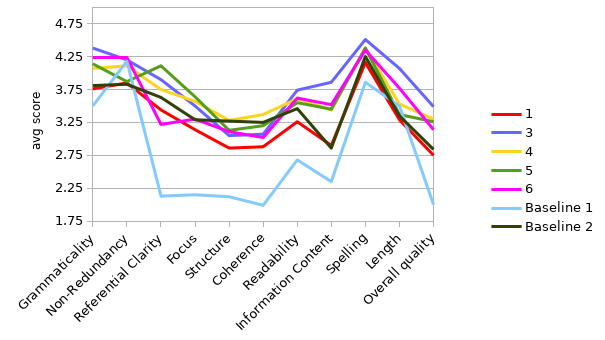
\includegraphics[width=0.8\linewidth]{figures/quality_per_category.png}
\end{figure}  


Compared to the other groups our system performs in average 0.245 to 0.67 points worse than the other systems in all evaluation  categories, having the biggest difference in information content. A comparative overview over all categories can be found in figure \ref{fig:quality_per_category}. A detailed analysis of the category scores can be found in the next paragraph \ref{analysis_by_topics}.

\subsubsection{Analysis by topics}
\label{analysis_by_topics}

Our system has an average overall quality of 2.75 with a standard deviance of 0.80. In figure \ref{fig:quality_per_topic} it can be seen that the the overall quality varies a lot and ranges from bad summaries (1.5 points) to excellent summaries (4.75 points). Our best summary according to the overall quality score is about potty training (topic 1048). This summary is indeed very good since it only contains advice about potty training and does not contain redundant information (see \ref{best_summary}). The worst summary concerning overall quality contains two almost exactly identical sentences which only differ in one word "children"/"kids" (see \ref{worst_summary})

\begin{figure}[!ht]
	\centering
	\label{fig:quality_per_topic}
	\caption{Average overall quality per topic}
	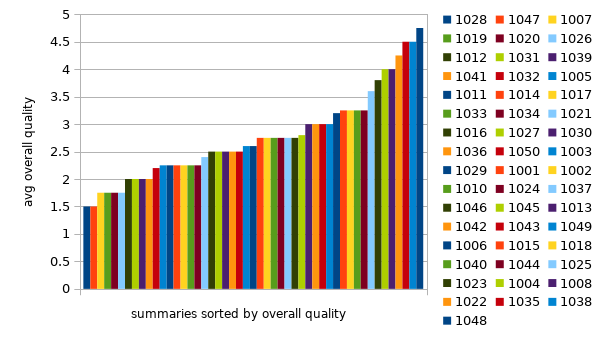
\includegraphics[width=0.8\linewidth]{figures/quality_per_topic.png}
\end{figure}

\begin{figure}
	\caption{Best summary by overall quality}
	\label{best_summary}
	\noindent\fbox{%
		\parbox{\textwidth}{%
			Begin potty training when you are ready to devote the time and energy to encourage your child on a daily basis for at least three months.
			When your child is ready, he will signal that his diaper is wet or soiled or will tell you that he would like to go to the potty.
			Tell your child that the potty chair is his own chair.
			Stay with your child when he is on the potty chair.
			Place your child on the potty chair whenever he signals the need to go to the bathroom so he'll associate the potty with the urge to go.
		}%
	}	
\end{figure}

\begin{figure}
	\caption{Worst summary by overall quality}
	\label{worst_summary}
	\noindent\fbox{%
		\parbox{\textwidth}{%
			For most children school is where they start to really develop their own personalities away from their families; interacting with others from different backgrounds without parents' interference.
			For most kids school is where they start to really develop their own personalities away from their families; interacting with others from different backgrounds without parents' interference.
		}%
	}	
\end{figure} 


\subsubsection{Analysis by evaluation categories}
Most categories seem like regular text evaluation categories like spelling and grammaticality. Other categories seem especially summary-related. These are the categories information content and focus. They represent the goal of a summary very well which is to present the most important content of the summarized texts. Since all summarized texts in this corpus are about a certain query the focus should be important, too.

The resulting evaluations can be used for assessing the quality of the summaries produced by our system. It is important for the evaluation that we only worked on the nugget extraction. Our results were given to another group which then produced the summaries. In this way we are completely responsible for the results in some evaluation categories while other evaluation results also depend on the steps of  building the hierarchy and actually creating a summary. The output we gave to the other group were whole sentences
% (more about the output in section ...).
The summary is then only built out of these sentences. In this way all categories which just operate on a sentence level are completely our responsibility. Among these categories are strictly only the two categories "Spelling" and grammaticality. We are also highly responsible for the categories information content, focus and non-redundancy. All extracted sentences should ideally contain important information related to the query. Furthermore it can be argued that in the step of nugget extraction nuggets with the same meaning as another nugget are ignored. The categories referential clarity, structure and coherence in comparison are very dependent on the ordering of the sentences. It can be argued that referential clarity is also influenced by the nugget extraction. For sentences with a pronoun the system should also extract the reference sentence. Otherwise the sentence is not well usable in the next steps. This is not done in the step of nugget extraction, but in later steps. The category length depends especially on the last step, the summary creation. Readability and of course information content are very general categories which can't be assigned to any particular step. The focus of our analysis will be all steps which can be influenced by our work, the nugget extraction. Thus the categories structure, length and coherence will only be shortly discussed.

\paragraph{Grammaticality}
Since we use only full sentences for the creation of the summaries it is surprising that the results in "Grammaticality" and "Spelling" are not near the maximum score. The comments of the annotators hint at certain repeatedly made mistakes. Many of them are related to the fact that the source texts are taken from forum posts which can contain mistakes like this. Some sentences contain punctuation error like missing dots or quotes. Annotators criticize incomplete sentences like "The study of mechanical self propulsion in vehicles." which often seem like headlines.  There are also summaries which consist of only one long sentence like "Developing performance-enhancing behavioral therapies for individuals prenatally exposed to alcohol and focusing remediation efforts on disabilities that affect quality of life and everyday functioning Information about illicit drugs, alcohol, prevention and treatment programs can be obtained on the following websites: Being raised in a family where abuse of alcohol or other substances (illegal drugs or prescription medications) occurs can lead to a host of challenges for children." All these problems can be solved in different ways. A possible solution for punctuation errors is to check if a sentence ends with a punctuation sign and to check if parentheses and quotes are properly closed. For the removal of incomplete sentences a POS tagger can be used. It should check if a sentence contains at least a noun and a verb. Extremely long sentences can be just filtered out with a certain threshold length. In this way also too short sentences which can also cause problems could be filtered out.

\paragraph{Spelling}
Now we take a look at different errors in the category "Spelling". This category contains some punctuation errors, too. It seems like annotators do not know in which category these kinds of errors belong. In this case the annotation protocol needs to be specified. A mistake unique to the category "Spelling" is incorrect upper- and lowercasing. Another mistake is wrong white spacing, like in "loans , you". The upper- and lowercasing could be handled by a POS tagger so that only proper names are uppercased and everything else is lowercased. Additional white spaces can be easily removed with a regular expression.

As we see the categories grammaticality" and spelling contain many mistakes which can be fixed quite easily. That means that actual improvement in these categories could be achieved.

\paragraph{Information Content}
"Information Content" is one of our system's greatest weaknesses. Annotators' comments point towards the relatedness of "Information Content" and "Non-Redundancy", "Focus" and "Readability". The correlation of "Information Content" with the other categories calculated with Pearson's r shows that information content is indeed most related to focus (0.52) and readability (0.5), but the relationship with non-redundancy (0.27) is surprisingly low.
%(!!! Reference to a graphic).
Thus, to gain better results in information content it is important to optimize focus and readability.

\paragraph{Focus}
The score in focus of 3.14 is much better than of baseline 1 (2.15) but slightly worse than the score in "Focus" of baseline 2. We integrate the query in our nugget extraction by averaging the query with a nugget. It seems like we need additional features to incorporate the query. This should be a focus of future work.

\paragraph{Non-Redundancy}
The results of our system in "Non-Redundancy" are worse than the ones of baseline 1 but similar to the results of group 5 and baseline 2. The similarity to group 5 is very interesting since we used their pipeline after the nugget extraction from this group. It hints that group 5's system does not properly remove duplicates while creating a summary. An extreme example is the following summary which consists of four sentences with a content nearly identical: "Computer Explorers uses innovative and creative ways to excite young learners about science, technology, engineering and math subjects. The local Computer Explorers uses technology in creative ways to engage students in science, math, English and other core academic subjects. Computer Explorers is an education company that uses technology in creative ways to engage students in science, math, English and other core academic subjects. Computer Explorers is a local education company that uses technology in innovative ways to engage students in science, math, English and other core academic subjects". It seems like no similarity detection is used. This does not necessarily have to be done in summary creation but can be also done in the nugget extraction, at least if full sentences are extracted.

\paragraph{Readability}
Our system's readability score is worse than the readability scores of the other groups and baseline 2, but better than baseline 1. Readability is a measure which is quite subjective and hard to define. It depends on other categories like grammaticality, spelling and structure. We calculate the Pearson's r to find out which evaluation categories influence readability the most. Readability correlates highest with grammaticality (0.52), followed by information content (0.5), structure and coherence (both 0.45).   

\paragraph{Structure and Coherence}
The results in structure and coherence exceed baseline 1 but are worse than baseline 2 and the other groups. Group 5 whose pipeline we partially used performs approximately 0.3 points better at each category only by using different nuggets. It seems like the results of these categories can be already improved through better nugget extraction. Additional improvements have to be done in further steps of the pipeline which is not the focus of our work.

\paragraph{Overall Quality}
A category which we have not discussed yet is the category overall quality". We see it as a final assessment of the summary which summarizes all other categories. The average overall score of our summary is 2.75. This is 0.39 to 0.74 points worse than the average overall score of the other groups. Comparing with the baselines our system performs much better than baseline 1 but slightly worse than baseline 2. We now take a look at what categories have the greatest impact on the overall quality of a summarization. Supposedly categories which are strongly summary-specific, namely information content and focus have a high correlation with overall quality. As a correlation measure we use Pearson's r and compute the correlation of the overall quality to all other categories (see figure \ref{fig:corr_overall_quality}).

\begin{figure}
	\centering
	\label{fig:corr_overall_quality}
	\caption{Correlation between overall quality and the other evaluation categories}
	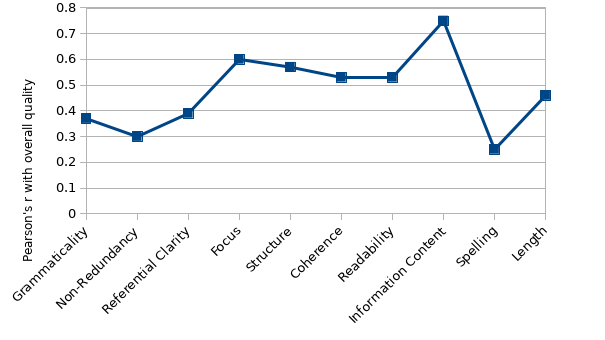
\includegraphics[width=0.8\linewidth]{figures/correlation_overall_quality.png}
\end{figure}

The strongest correlation has indeed "Information Content" with 0.75. The categories which are also very important for the overall quality are "Focus"(0.6), "Structure"(0.57), "Readability"(0.53) and "Coherence"(0.53). The annotators had to assign weights for each category in each evaluation. In this way they could express which categories they think are most important for a summary. The categories which they named in average as most important are "Information Content" (4.14), "Focus" (3.68) and "Readability" (3.47). These values match the calculated correlations. Interestingly, the annotators ranked "Non-Redundancy" in the midfield as an important category for overall quality while the correlation shows that it actually has the second-smallest effect on the overall quality. The least impact on the overall quality has the spelling of a summary. In conclusion especially "Information Content", "Focus" and "Readability" need to be improved to gain a higher overall summary quality.